\chapter{General Architecture}
\label{chap:gen-arch}

\section{Resulting Architecture}
\label{chap:architecture-overview}

The result of combining \textbf{MIG} and \textbf{DRA} is a layered architecture that separates the physical organization of the accelerator from the way applications request it. This separation is particularly important for GPUs: although MIG determines which devices physically exist, a tenant should not need to identify a particular GPU or MIG UUID in its Pod specification. Instead, the application declares the characteristics of the resource it requires, while the infrastructure selects and prepares a compatible device.

\begin{figure}[H]
    \centering
    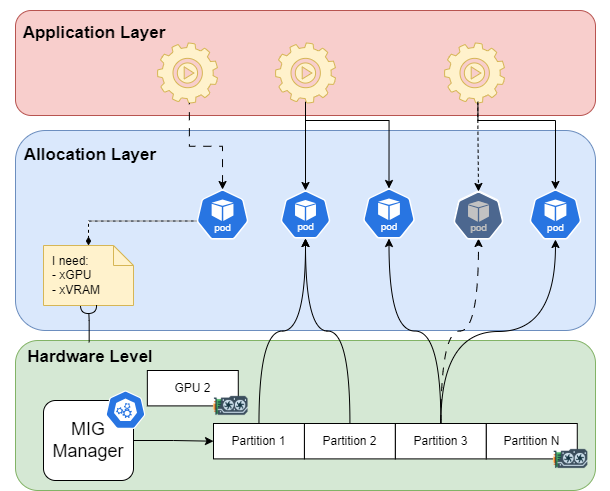
\includegraphics[width=0.65\textwidth]{images/DRA_MIG_Architecture.drawio}
    \caption{MIG + DRA Architecture Overview}
    \label{fig:mig-dra-logical-architecture}
\end{figure}

Table~\ref{tab:logical-architecture} summarizes the resulting logical architecture. The hardware and allocation layers jointly form the \emph{infrastructure layer}; the application layer consumes the capabilities exposed by that infrastructure.

\begin{table}[htbp]
    \centering
    \small
    \caption{Logical layers of the implemented GPU platform.}
    \label{tab:logical-architecture}
    \begin{tabularx}{\textwidth}{@{}p{0.18\textwidth}p{0.17\textwidth}X@{}}
        \toprule
        \textbf{Macro-layer} & \textbf{Layer} & \textbf{Responsibility} \\
        \midrule
        Application & Application & Runs tenant workloads directly or through higher-level frameworks that coordinate their execution. \\
        Infrastructure & Allocation & Translates declarative device requirements into the allocation and preparation of a compatible resource for a Pod. \\
        Infrastructure & Hardware & Controls the physical accelerator and the set of GPU devices that can be allocated by the upper layer.\\
        \bottomrule
    \end{tabularx}
\end{table}

At the bottom, the \emph{hardware layer} manages the accelerator as a node resource, this means that a requested node configuration determines which GPU Instances exist and therefore which combinations of compute and memory can be exposed. This responsibility is analogous to node-level resource provisioning: it establishes the capacity available to the cluster, but does not decide which AI application should receive it.

Immediately above it, the \emph{allocation layer} provides the decoupling introduced by DRA. From the perspective of a Pod, a request can express a requirement such as ``one NVIDIA MIG device satisfying these conditions'', rather than naming a physical instance. The NVIDIA DRA driver publishes the device inventory through ResourceSlices, while DeviceClasses and claim selectors describe the acceptable resources. During scheduling, Kubernetes chooses a node and a compatible device, then the node-side DRA component prepares that device and makes it available to the container. As a result, hardware layout and application manifests can be reasoned about separately, provided that the inventory contains a device satisfying the claim~\cite{kubernetes135dra,nvidia2026dradriverarchitecture}.

These two layers constitute an \textbf{application-agnostic} infrastructure. In this context, \emph{application-agnostic} does not mean that the infrastructure ignores application requirements: those requirements are explicitly carried by claims. It means that the infrastructure does not need to understand model semantics, prompts, or inference-server internals, and is not constructed for a single application. Its contract is expressed in resource properties.

The highest level is the \emph{application layer}. A tenant can deploy a Pod that consumes DRA claims directly or use an intermediate framework. For example Kueue can add queueing and admission control for finite jobs or KubeRay can coordinate distributed Ray applications. These components do not replace the infrastructure layers: they decide when and how application work should run, then rely on Kubernetes and DRA to satisfy the corresponding device requests.

\paragraph{Lifecycle.} The end-to-end path can therefore be summarized as follows:

\begin{enumerate}
    \item \textbf{MIG Manager} reconciles the requested MIG geometry and creates the allocatable hardware partitions.
    \item \textbf{The NVIDIA DRA driver} discovers those partitions and publishes their attributes and capacities to Kubernetes.
    \item \textbf{A Pod}, either directly or through an intermediate framework, references a ResourceClaim or ResourceClaimTemplate that describes an acceptable device.
    \item \textbf{Kubernetes} selects a compatible device and node, after which the DRA driver prepares the allocation and exposes it to the container.
\end{enumerate}

\section{Evaluating MIG and DRA: Proof-of-Concept Progression}
\label{sec:poc-progression}

The experimental work is organized as two successive proofs of concept rather than as two unrelated deployments. Both use the infrastructure described above, but each isolates a different question about the combination of MIG and DRA.

The first proof of concept investigates \emph{spatial consolidation}. It asks whether several lightweight inference-server instances can use one physical A100 more effectively when each instance is placed on an isolated MIG partition. The comparison separates two effects: the performance loss caused by restricting one server to a smaller device, and the aggregate gain that may be obtained by executing several servers in parallel. DRA supplies each Pod with a MIG device through a claim, but the device remains attached for the Pod's lifetime. In this design, DRA is therefore a declarative provisioning mechanism: it does not continuously adapt the allocation to incoming inference requests.

This observation motivates the second proof of concept. A long-running inference server makes only one allocation decision when it starts, so its results cannot demonstrate a performance advantage caused by repeated DRA decisions. The second experiment consequently moves to finite batch workloads managed by Kueue. Devices are released when jobs finish, allowing subsequent jobs to express flexible requirements and to be assigned to whichever compatible partition becomes available. The progression first evaluates whether MIG-based consolidation is beneficial, then evaluates whether DRA's richer allocation semantics can improve the use of a fixed heterogeneous device pool.

\section{From Workload Priority to GPU-Aware Service Classes}
\label{subsec:kueue-problem}

The first proof of concept exposes a distinction between dynamic device allocation and dynamic application demand. Each Ollama Pod obtains a device when it starts and then processes many inference requests using that same allocation. An HTTP request to the inference server is not a new ResourceClaim: the model-serving process continues to use the device already prepared for its container. Consequently, changes in request volume or request length do not cause Kubernetes to reconsider the assigned GPU.

DRA could still provide more granular selection at startup, for example by filtering memory capacity or compute resources. However, those conditions would be evaluated for the server's initial allocation, not repeatedly for its individual requests. In the first PoC, claims intentionally accept any MIG device, so even that finer selection is not exercised. The performance comparison therefore primarily concerns MIG geometry and workload consolidation, rather than DRA's ability to select among heterogeneous resources.

This limitation is characteristic of long-running services with persistent device assignments, including conventional LLM-serving Deployments. It is not an intrinsic restriction on language models: new replicas, restarts, or batch executions can introduce new allocation opportunities. Nevertheless, a continuously running server does not automatically translate its changing inference demand into repeated DRA decisions, and the experimental stack does not support resizing or exchanging its GPU in place~\cite{kubernetes135dra}.

A suitable second scenario must therefore contain recurring resource requests and releases. Finite Kubernetes Jobs provide this lifecycle naturally: a Job performs a bounded task, its Pods stop using the device when execution finishes, and the allocation can subsequently be reclaimed according to the Pod and claim lifecycle. Each new Job can request a compatible device from the inventory available at that time. Even when successive Jobs run the same program, a flexible claim can permit different devices as resources become free. The objective is to identify a specific policy under which this expressiveness yields measurable improvements in completion time or aggregate throughput. Such improvements would be an indirect consequence of better resource selection and reuse, not a computational acceleration inherently provided by DRA.

\subsection{Kueue as the Batch Admission Layer}
\label{subsec:kueue-admission-layer}

Kueue was selected because it adds Kubernetes-native queueing and quota management without replacing the existing scheduler or Job controller. It decides which workloads may start, which must wait, and, where configured, which may be preempted. Namespace-scoped LocalQueues connect submitted Jobs to cluster-level ClusterQueues, where administrators define resource quotas and admission policies. Pod placement and device preparation remain the responsibility of Kubernetes and the DRA driver~\cite{kueue2026overview}.

This division of responsibilities fits the proposed architecture: Kueue governs access to a shared pool, while DRA expresses which devices are acceptable for each admitted workload. In the ResourceClaimTemplate integration, Kueue maps DeviceClasses to logical quota resources through \texttt{deviceClassMappings} and can account for the requested device count. Admission verifies quota availability; it does not itself choose the physical MIG instance~\cite{kueue2026dra}. Kueue therefore provides an appropriate setting for evaluating repeated, policy-controlled allocations without requiring a custom queueing system.

\subsection{Beyond Admission Priority}
\label{subsec:gpu-aware-service-classes}

Kueue already supports workload priority through \texttt{WorkloadPriorityClass}, independently of Pod priority. This value influences queue ordering and, depending on configuration, preemption and competition for borrowed quota. Higher priority can favour earlier admission, but it does not determine how quickly an admitted Job executes. It does not select a larger GPU partition, increase the compute capacity of an assigned device, or accelerate CUDA kernels. A high-priority Job may therefore start earlier but still finish late if it runs on a slow or constrained resource. From the user's perspective, the relevant objective is often the total time between submission and completion, not admission time alone. That interval includes queueing, startup, execution, and completion overhead.

The proposed policy interprets a request for higher service priority as an interest in earlier completion. It therefore combines two complementary mechanisms:

\begin{itemize}
    \item \textbf{Admission priority}, supplied by Kueue, expresses the relative importance of starting the workload.
    \item \textbf{GPU eligibility constraints}, supplied by DRA, express which compute and memory resources may execute it.
\end{itemize}

Together, these define a \emph{GPU-aware service class}. For example, a Gold class can combine higher workload priority with a minimum compute requirement, allowing either a medium or a large compatible MIG device. A Bronze class can combine lower priority with eligibility for a smaller partition. This is a policy built from existing Kueue and DRA objects, not a new native Kueue API, an execution-time predictor, or a deadline guarantee.

The flexibility of the device requirement matters as much as its minimum capacity. Pinning every high-priority Job to one exact profile can leave another suitable partition idle while Jobs continue waiting. A broader eligibility condition allows subsequent Jobs to use whichever acceptable resource becomes available, without changing devices already assigned to running Jobs. This can reduce avoidable waiting and improve use of a heterogeneous pool.

The benefit remains workload-dependent: a larger partition is useful only if the application can exploit it, and waiting for a larger device can outweigh a shorter execution time. The proposed service classes must therefore be evaluated against explicit allocation baselines at comparable usable capacity. Any observed gain belongs to the combined admission and allocation policy, rather than proving that DRA alone always improves performance.
